%!TEX root = ../Thesis.tex
\chapter{Theory}

%!TEX root = ../Thesis.tex
\section{Feed forward Neural Network}
\label{sec:theory:ffnn}

Neural Machine Translation is based on the neural network framework. Modern networks are extreamly complex and uses rather advanced operations such as convolution, others uses complex combinations of simpler operations such as the LSTM block. To give a short introduction to this framework the feed forward neural network (FFNN) is presented. This is the simplest type in the neural network familiy. As such it doesn't have much use for translation, but the more advanced neural networks can be seen as extensions of a feed forward neural network.

\subsection{The neuron}

The neuron is the main component in any neural network. Mathematically it is just a function which takes a vector and returns a scalar. It does this by a weighted sum of the inputs $\{ x_i \}_{i=1}^I$ and by adding a bias value $b$. The sum is then then typically transformed using a non-linear function $\theta$.
\begin{equation}
a = \theta(z),\quad z = \sum_{i=1}^I w_{i} x_i + b
\end{equation}

The value $a$ is the output of the neuron and is called the \textit{activation}. In the past the sigmoid function $\sigma(\cdot)$ and the hyperbolic tangent $\tanh(\cdot)$ function have been very popular\cite{bishop}, but recently the rectified linear unit (ReLU) $\theta(z) = \max(0, z)$ has become the norm. If no non-linear function is applied then the identity function $\theta(a) = a$ is used.

\begin{figure}[H]
	\centering
	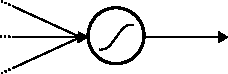
\includegraphics[scale=1]{theory/ffnn-neuron}
	\caption{Visual representation of a single neuron. The left arrows represents the input elements $\{ x_i \}_{i=1}^I$. The circle represent the function that returns the activation scalar $a$ (right arrow).}
\end{figure}

\subsection{The network}

A feed forward neural network is in its simplest form a \textit{multivariate non-linear regression model} constructed by combining neurons. Such a regression model can then be turned into a classification model by adding a softmax transformation \cite{the-elements-of-statistical-learning} to the output. By doing this each output value becomes the class probability $y_k = P(C_k | x)$.

\begin{figure}[h]
	\centering
	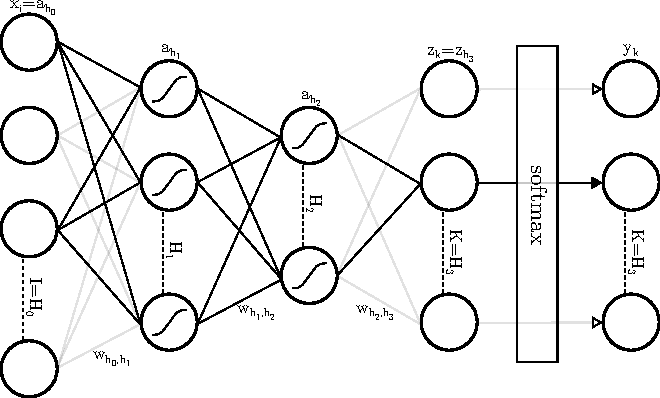
\includegraphics[scale=1]{theory/ffnn-network.pdf}
	\caption{Visual representation of a neural network with two hidden layers. Some lines are less visible, this is just a visual aid because the many connections can be difficult to look at.}
	\label{fig:theory:ffnn:network}
\end{figure}

The neural network in Figure \ref{fig:theory:ffnn:network}, have one input layer $x_i, i \in [1, I]$ and one output layer $y_k, k \in [1, K]$. This is the same for any neural network, what varies is the type of network (here a feed forward neural network) and the amount of hidden layers (here two). The hidden layers are typically the layers that contains the non-linear transformation functions. If there are no hidden layers, the neural network is just a multiclass logistic regressor\cite{bishop}.

Because there are more than one neuron in each layer and many layers, the neuron index and layer index is denoted by the subscript. For example a neuron output is denoted by $a_{h_{\ell}}$ for $h_{\ell} \in [1, H_{\ell}]$, where $h_{\ell}$ is the neuron index and $H_\ell$ is the amount of neurons in layer $\ell$.

\subsection{Forward pass}

Calculation of the network output ($y_k$) is sometimes called the \textit{forward pass}, while the parameter estimation is sometimes called the \textit{backward pass}.

The \textit{forward pass} is simply calculated by applying the neuron function to all nerons in all layers. By defining $a_{h_0} = x_i$ the \textit{forward pass} can be generalized to any amount of hidden layers ($L$):
\begin{equation}
\begin{aligned}
a_{h_\ell} &= \theta(z_{h_\ell}), && \forall h_{\ell} \in [1, H_{\ell}], \ell \in [1, L] \\
z_{h_\ell} &= \sum_{h_{\ell-1} = 1}^{H_{\ell-1}} w_{h_{\ell-1}, h_{\ell}} a_{h_{\ell-1}} + b_{h_{\ell}}, && \forall \ell \in [1, L+1] \text{ where: } a_{h_0} = x_i, H_0 = I \\
\end{aligned}
\end{equation}

Note that the last layer $\ell = L + 1$ does not use the non-linear transformation function $\theta$, instead it uses the softmax function.
\begin{equation}
\begin{aligned}
y_k = \frac{\exp(z_k)}{\sum_{k'=1}^K \exp(z_{k'})}, && \forall k \in [1, K] \text{ where: } z_k=z_{h_{L+1}}, K = H_{L + 1}
\end{aligned}
\label{eq:theory:ffnn:y}
\end{equation}

The $z_k$ values there are feed to the softmax function are often called \textit{logits}, because they are unnormalized log properbilities ($\exp(z_k) \propto y_k$). This has some advantages, for example if one wants the most likely label given $\mathbf{x}$ one can just find the largest $z_k$ and thus skip the softmax, which can otherwise be quite expensive to calculate.

\subsection{Loss function}

Optimization of the parameters $w_{i,j}$ and $b_{j}$ requires definition of a loss function. For classification it makes sense to maximize the joint probability of observing all the observations:
\begin{equation}
P(\mathbf{t} | \mathbf{x}, \mathbf{w}, \mathbf{b}) = \prod_{n=1}^N P(\mathbf{t}_n | \mathbf{x}_n, \mathbf{w}, \mathbf{b})  = \prod_{n=1}^N \prod_{k=1}^K P(C_{n, k} | \mathbf{x}_n, \mathbf{w}, \mathbf{b})^{t_{n, k}}
\end{equation}

Here $\mathbf{x}_{n}$ is the input vector for observation $n$, with a corresponding label vector $\mathbf{t}_n$. The label vector is an indicator vector constructed using 1-of-K encoding. The class probability $P(C_{n, k} | \mathbf{x}_n, \mathbf{w}, \mathbf{b})$ is $y_k$ from the \textit{forward pass} for observation $n$.

The logarithm is then used to create linearity and avoid numerical floating point issues. The sign is also changed such that it becomes a loss function:
\begin{equation}
- \ln\left(P(\mathbf{t} | \mathbf{x}, \mathbf{w}, \mathbf{b})\right) = - \sum_{n=1}^N \sum_{k=1}^K t_{n, k} \ln\left( P(C_{n, k} | \mathbf{x}_n, \mathbf{w}, \mathbf{b})\right)
\label{eq:theory:ffnn:long-loss}
\end{equation}

Because of the linearity in \eqref{eq:theory:ffnn:long-loss} it makes sense to just consider the loss function for one datapoint, thus the $n$ index can be omitted. This gives the final loss function which is denoted by $\mathcal{L}$:
\begin{equation}
\mathcal{L} = - \sum_{k=1}^K t_{k} \ln\left( P(C_{k} | \mathbf{x}, \mathbf{w})\right) =  - \sum_{k=1}^K t_k \ln(y_k)
\label{eq:theory:ffnn:loss}
\end{equation}

The formulation \eqref{eq:theory:ffnn:loss} is particularly useful as it allows for some numerical stability tricks, see Appendix \ref{appendix:numerical-stability:cross-entropy} \todo{\url{https://github.com/tensorflow/tensorflow/blob/master/tensorflow/core/kernels/sparse_xent_op.h\#L190L219}}.

\subsection{Backward pass}

For the neural network there is no closed form solution to optimizing the loss function. Instead gradient based optimization algorithms are used. Gradient based optimization uses the derivatives of the loss function with respect to the parameters to iteratively optimize the parameters. This approach will be discussed in Section \ref{sec:theory:optimization}, for now the important part is calculate the derivatives:
\begin{equation}
\begin{aligned}
\frac{\partial \mathcal{L}}{\partial w_{h_{\ell-1}, h_\ell}} \wedge \frac{\partial \mathcal{L}}{\partial b_{h_\ell}}, && \forall \ell \in [1, L + 1]
\end{aligned}
\label{eq:theory:ffnn:bprop-problem}
\end{equation}

For calculating the derivatives the \textit{error backpropagation} algorithm is used, this algorithm results in what is called the \textit{backward pass}.

The main trick in \textit{error backpropagation} is to define the partial derivative $\delta_{h_\ell}$, this is then used for bookkeeping and is what makes it feasiable to calculate the derivatives.
\begin{equation}
\delta_{h_\ell} \defeq \frac{\partial \mathcal{L}}{\partial z_{h_\ell}}
\end{equation}

Using this defintion the chain rule can be applied on \eqref{eq:theory:ffnn:bprop-problem}:
\begin{equation}
\begin{align}
\frac{\partial \mathcal{L}}{\partial w_{h_{\ell-1}, h_\ell}} &= \frac{\partial \mathcal{L}}{\partial z_{h_\ell}} \frac{\partial z_{h_\ell}}{\partial w_{h_{\ell-1}, h_\ell}} &&= \delta_{h_\ell} a_{h_{\ell-1}},&& \forall \ell \in [1, L+1],\quad a_{h_0} = x_i \\
\frac{\partial \mathcal{L}}{\partial b_{h_\ell}} &= \frac{\partial \mathcal{L}}{\partial z_{h_\ell}} \frac{\partial z_{h_\ell}}{\partial b_{h_\ell}} &&= \delta_{h_\ell},&& \forall \ell \in [1, L+1]
\end{align}
\end{equation}


Calculating $\delta_{h_\ell}$ is a bit more involved since $z_{h_\ell}$ affects more than one intermediate variable, but even so the chain rule can still be applied:
\begin{equation}
\begin{aligned}
\delta_{h_\ell} = \frac{\partial \mathcal{L}}{\partial z_{h_\ell}} &= \frac{\partial \mathcal{L}}{\partial a_{h_\ell}} \frac{\partial a_{h_\ell}}{\partial z_{h_\ell}} \\
&= \theta'(z_\ell) \sum_{h_{\ell+1}}^{H_{\ell+1}} \frac{\partial \mathcal{L}}{\partial z_{\ell+1}} \frac{\partial z_{\ell+1}}{\partial a_\ell} \\
&= \theta'(z_\ell) \sum_{h_{\ell+1}}^{H_{\ell+1}} \delta_{h_{\ell+1}} w_{h_\ell, h_{\ell+1}}, \forall \ell \in [1, L]
\end{aligned}
\label{eq:theory:ffnn:bprop}
\end{equation}

The last delta $\delta_{h_{L+1}}$ is diffrent but can still be calculated by using the chain rule.
\begin{equation}
\delta_{h_{L + 1}} = \delta_k = \frac{\partial \mathcal{L}}{\partial z_k} = \sum_{k'=1}^K \frac{\partial \mathcal{L}}{\partial y_{k'}} \frac{\partial y_{k'}}{\partial z_k}
\label{eq:theory:ffnn:bprop-deltaK}
\end{equation}

The first derivative $\frac{\partial \mathcal{L}}{\partial y_{k'}}$ can be derived from \eqref{eq:theory:ffnn:loss}:
\begin{equation}
\frac{\partial \mathcal{L}}{\partial y_{k'}} = \frac{\partial}{\partial y_{k'}} \left(- \sum_{k''=1}^K t_{k''} \ln(y_{k''})\right) = -\frac{t_{k'}}{y_{k'}}
\label{eq:theory:ffnn:bprop-Ldy}
\end{equation}

The other derivative $\frac{\partial y_{k'}}{\partial z_k}$ can be derived from \eqref{eq:theory:ffnn:y}:
\begin{equation}
\begin{aligned}
\frac{\partial y_{k'}}{\partial z_k}
&= \frac{\partial}{\partial z_k} \frac{\exp(z_{k'})}{\sum_{k''=1}^K \exp(z_{k''})} \\
&= \frac{\frac{\partial}{\partial z_k} \exp(z_{k'})}{\sum_{k''=1}^K \exp(z_{k''})}
- \frac{\exp(z_{k'}) \frac{\partial}{\partial z_k} \sum_{k''=1}^K \exp(z_{k''})}{\left(\sum_{k''=1}^K \exp(z_{k''})\right)^2} \\
&= \frac{\frac{\partial}{\partial z_k} \exp(z_{k'})}{\sum_{k''=1}^K \exp(z_{k''})}
- \frac{\exp(z_{k'})}{\sum_{k''=1}^K \exp(z_{k''})} \frac{\frac{\partial}{\partial z_k} \sum_{k''=1}^K \exp(z_{k''})}{\sum_{k''=1}^K \exp(z_{k''})}
\end{aligned}
\end{equation}

Because of the difference in index, the first term is only not zero when $k = k'$, in which case $y_k$ is the derivative. It thus becomes useful to define:
\begin{equation}
\delta_{i,j} = \begin{cases}1& \text{when } i = j \\ 0 & \text{otherwise}\end{cases}
\end{equation}

Similarly in the second term $\frac{\partial}{\partial z_k} \exp(z_{k''})$ is zero except in the case where $k = k''$:
\begin{equation}
\frac{\partial y_{k'}}{\partial a_k} = \delta_{k, k'} y_k - y_{k'} y_k
\label{eq:theory:ffnn:bprop-yda}
\end{equation}

The result from \eqref{eq:theory:ffnn:bprop-Ldy} and \eqref{eq:theory:ffnn:bprop-yda} is then combined into \eqref{eq:theory:ffnn:bprop-deltaK}:
\begin{equation}
\begin{aligned}
\delta_{h_{L + 1}} = \delta_k &= \sum_{k'=1}^K -\frac{t_{k'}}{y_{k'}} \left( \delta_{k, k'} y_k - y_{k'} y_k \right) = \sum_{k'=1}^K -\frac{t_{k'}}{y_{k'}} \delta_{k, k'} y_k + \sum_{k'=1}^K \frac{t_{k'}}{y_{k'}} y_{k'} y_k \\
&= -\frac{t_k}{y_k} y_k + y_k \sum_{k'=1}^K t_{k'} = -t_k + y_k = y_k - t_k
\end{aligned}
\label{eq:theory:ffnn:bprop-deltaKfinal}
\end{equation}

To get $\sum_{k'=1}^K t_{k'} = 1$ it's used that $\{ t_{k'} \}_{k'=1}^K$ is the target distribution and thus must sum to 1.

Using \eqref{eq:theory:ffnn:bprop-deltaKfinal} and \eqref{eq:theory:ffnn:bprop} all $\delta_{h_\ell}$ for $\ell \in [1, L+1]$ can be calculated for a feed forward neural network with $L$ hidden layers. Note how \eqref{eq:theory:ffnn:bprop-deltaKfinal} is an error measure and this value is propagated back through the network by the $\delta_{h_\ell}$ equations in \eqref{eq:theory:ffnn:bprop}. This is why the method is called \textit{error backpropagation}.

\clearpage

\section{Gradient Based Optimization}
\todo[inline]{Section describing gradient descent and more advanced algorithms, such as adam optimization.}
\subsection{Gradient Descent Optimization}
\subsection{Adam Optimization}
\clearpage

\section{Convolution Neural Network}

Convolution is typically used in signal and image processing, but has recently found its way to machine learning in neural networks. A classical example is image blurring, where one is given an image $a(x, y)$ which is to be blurred. This blurring is done by averaging neighboring pixels, this average is typically weighted using a 2D Gaussian distribution.

This can be generalized to any input $a(x, y)$ and any weight function $w(x, y)$ by:
\begin{equation}
z(x, y) = (a * w)(x, y) = \int_{-\infty}^\infty \int_{-\infty}^\infty a(i, j) w(x - i, y - j) \partial i \partial j
\end{equation}

Similarly for a discrete image and discrete weight function:
\begin{equation}
z(x, y) = (a * w)(x, y) = \sum_{i = -\infty}^\infty \sum_{j = -\infty}^\infty a(i, j) w(x - i, y - j)
\end{equation}

Both the continues and discrete formulation has some interesting mathematical properties, the convolution operator ($*$) is both commutative and associative. There is also the convolution theorem which combines convolution with the Fourier transformation. While these properties are useful in theoretical work, they have little use in neural networks, it is more the idea behind convolution that is used. In practise network networks uses a finite kernel matrix $w$, and input image $a$. Furthermore most frameworks uses the cross-correlation operator instead of the convolution operator, the difference being that the kernel matrix is flipped. The operation is still called convolution among these frameworks, this wording is also adopted here and will be used for the rest of the thesis.
\begin{equation}
z(x, y) = (a * w)(x, y) = \sum_{i,\ j} a(x + i, y + j) w(i, j)
\end{equation}

Finally this thesis uses text as an input which only has one dimension, thus a 1D-convolution is used.
\begin{equation}
z(t) = (a * w)(t) = \sum_{i} a(t+r\,i) w(i)
\end{equation}

Convolution has shown to be a very powerful construct, this is primarily because of its locality and its parameter sharing. Locality means that one \textit{pixel} in the output layer only depends on a few \textit{pixels} in the input layer. This makes convolution fast to compute and reasonably easy to parallelize on a GPU. Parameter sharing means that one weight scalar in $w$ is affected by many input and output \textit{pixel}, this causes there to be a lot more data to estimate and optimize the parameter.

\subsection{Padding}
Having a finite input image raises the question on how to deal with the boundaries, where the kernel uses undefined data. In convolutional neural networks the typical strategy is to either restrict the output image such that all the data is known, this is known as the ``valid'' approach. Alternatively one can add a zero padding to the input image, such that the valid output image of the extended input image has the same size size as the original input image, this is known as the ``same'' approach. Finally there is the ``full'' approach where the input image is zero padded as much as what is meaningful. The ``full'' approach is rarely used in neural networks.

\begin{figure}[h]
	\centering
	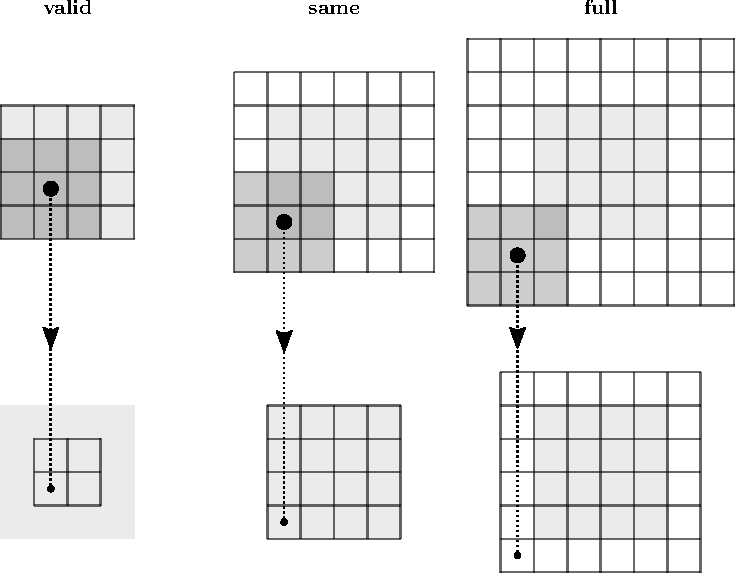
\includegraphics[scale=1]{theory/convolution-padding}
	\caption{Shows 3 padding strategies, known as ``valid'', ``same'', and ``full''.}
	\label{fig:convolution:padding}
\end{figure}

The ``valid'' padding approach is great because it doesn't assume anything about the data, that zero is an appropriate padding value. On the other hand it makes the output image small which limits the amount of convolutional layers one can apply.

The ``same`` padding approach is great because it doesn't change the output size, however zero may not be an appropriate padding value. In the ByteNet model presented later ``same`` padding is used because it doesn't change the image size, this is a requirement by residual learning which will also be discussed later.

\subsection{Channels}
Ordinary images a separated into 3 colors, red, green, and blue. This concept is generalized to what is called ``channels'', each color is one channel. A convolution will then merge the all channels into a new output image. For the output to have more than one channel, more than one convolution can be applied for each layer. This can be expressed as:
\begin{equation}
z_{h_\ell}(t) = (a_{\ell-1} * w_{:, h_\ell})(t) = \sum_{h_{\ell-1}}^{H_{\ell-1}} \sum_{i} a_{h_{\ell-1}}(t + i) w_{h_{\ell-1}, h_\ell}(i), \quad \forall h_\ell \in [1, H_\ell]
\end{equation}
where $h_{\ell-1} \in [1, H_{\ell-1}]$ denotes the channel on the input image and $h_\ell \in [1, H_\ell]$ is the channel on the output image.

The use of channels causes a very big increase in the number of parameters, if $w$ has the size $W$ without channels, it now has the size $W \times H_{\ell-1} \times H_\ell$. This increase may seam absurd but in practise channels are extremely powerful. The typical behaviour in convolutional neural networks is that each channel will represent some concept. In the first layer each channel may represent edges in different directions. In the second layer these edges may be combined to shapes, such as circular, rectangular, etc.. The last layers may represent ears, noses and hair, which is finally merged into faces. Neuroscientific research suggests that this is somewhat similar to what is happening in the human brain \cite[chapter 9.10]{deep-learning}.

Similarly for text we can imagine that letters are transformed into words and words into linguistic meaning. Unfortunately these transformations are much harder to visualize with text as input, thus whether or not this is actually what is happening remains unknown.

\subsection{Dilated Convolution}

Dilated convolution, also called atrous (with hole) convolution, is an extension on the convolution operator which makes the convolution kernel sparse. The sparseness is described with a dilation rate ($r$), a higher dilation rate means that the kernel is more sparse. A dilated convolution kernel ($w_r$) can be transformed to a dense convolution kernel $w$ by using the Kronecker product (denoted with $\otimes$).
\begin{equation}
w = w_r \otimes \begin{bmatrix}
1      & 0      & \cdots & 0      \\
0      & 0      &        & \vdots \\
\vdots &        & \ddots & \vdots \\
0      & \cdots & \cdots & 0
\end{bmatrix}
\end{equation}

The right hand side matrix in the Kronecker product is a mostly-zero matrix of size $r \times r$ with just a single $1$ in the top left element. The kernel matrix $w$ is visualized in Figure \ref{fig:convolution:dilation}.

\begin{figure}[h]
	\centering
	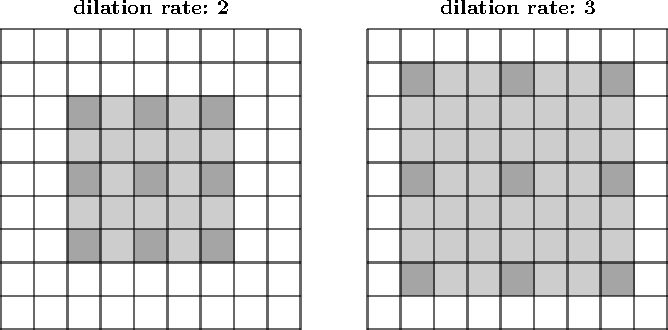
\includegraphics[scale=1]{theory/convolution-dilation}
	\caption{Shows dilated kernel with dilation rate $r = 2$ and $r = 3$.}
	\label{fig:convolution:dilation}
\end{figure}

Obviously converting the sparse kernel to a sense kernel with the Kronecker product is not a every computational efficient implementation. Instead the convolution (cross-correlation) operator can be modified to support dilation directly.
\begin{equation}
z(x, y) = (a *_r w)(x, y) = \sum_{i,\ j} a(x + r\, i, y + r\, j) w(i, j)
\end{equation}

While dilated convolution doesn't seam particularly useful as is, it becomes extremely powerful when multiple dilated convolution layers are stacked. For example if the first layer has no dilation ($r = 1$) and a kernel size of $3 \times 3$, and the second layer has a dilation rate of 3 ($r = 3$) with same kernel size ($3 \times 3$), the visible area of the second layer becomes much larger. This idea is called ``hierarchical dilated convolution'' and is the driving concept in the ByteNet model, which will be discussed and used later (section \ref{sec:theory:bytenet:hierarchical-dilated-convolution}).

For 1D convolution and with channels this can be expressed as:
\begin{equation}
z_{h_\ell}(t) = (a_{\ell-1} *_r w_{:, h_\ell})(t) = \sum_{h_{\ell-1}}^{H_{\ell-1}} \sum_{i} a_{h_{\ell-1}}(t + r\,i) w_{h_{\ell-1}, h_\ell}(i), \quad \forall h_\ell \in [1, H_\ell]
\label{eq:theory:convolution:final-forward}
\end{equation}

The backward pass for \eqref{eq:theory:convolution:final-forward} is derived in appendix \ref{appendix:backward-pass:dilated-convolution}.

\clearpage

\section{Initialization}
\todo[inline]{Section describing the vanishing and exploding gradient (moment) problem, and show to solve it using initialization.}
\clearpage

\section{Improving Convergence Speed}
\label{sec:convergence}

A good optimization algorithm is essential for fitting a deep neural network, however the convergence rate can often be improved by modifying the network architecture itself such that the cost function is easier to optimize. These modifications do not radically alter the network, but rather modifies existing layers. The modifications can become the identity function through parameter optimization and thus doesn't change the theoretical capabilities of the neural network.

\subsection{Batch Normalization}
Traditionally in feed forward neural networks, it has been the norm to standardize the input to have zero mean and unit variance.
\begin{equation}
\hat{x}_i = \frac{x_i - \mathbb{E}[x_i]}{\sqrt{\textsc{Var}[x_i] + \epsilon}}, \quad \forall i \in [1, I]
\end{equation}

This standardization places the input to the sigmoid activation function in its linear domain ($\sigma(\epsilon) \approx \epsilon, \forall \epsilon \in [-1, 1]$), which is a reasonable starting point for the optimization \todo{[LeCun et al., 1998b; Wiesler \& Ney, 2011]}. Batch normalization extends this idea to standardize before all activation functions in a deep neural network. This has positive consequences beyond limiting the sigmoid activation to its linear domain \cite{batch-normalization}.

Consider a neural network with just one hidden layer:
\begin{equation}
\mathcal{L}(\mathbf{t}, \mathbf{W}_2 \theta(\mathbf{W}_1 \mathbf{x} + \mathbf{b}_1) + \mathbf{b}_2)
\end{equation}
When optimizing the loss function, the parameters $\mathbf{W}_1, \mathbf{W}_2, \mathbf{b}_1$ and $\mathbf{b}_2$ are all optimized simultaneously. Furthermore, the optimization of $\mathbf{W}_2, \mathbf{b}_2$ does directly depend on $\theta(\mathbf{W}_1 \mathbf{x} + \mathbf{b}_1)$ though the error term. This becomes an issue when the distribution of $\theta(\mathbf{W}_1 \mathbf{x} + \mathbf{b}_1)$ changes because the updated $\mathbf{W}_2$ and $\mathbf{b}_2$ assumes the original distribution. This change of the distribution of the internal activations is called an \textit{internal covariate shift}. \cite{batch-normalization}.

The \textit{internal covariate shift} issue can be illustrated by considering a scalar $a = w x + b \sim \mathcal{N}(b, w)$, as it would appear in a very simple neural network, the sigmoid activation function is then applied on $\mathcal{N}(b, w)$ by using the \textit{change of variable theorem}. Using this one can change $w$ and $b$ and observe how the sigmoid activation distribution changes (Figure \ref{fig:convergence:batch-norm:activation-distribution}).

\begin{figure}[h]
	\centering
	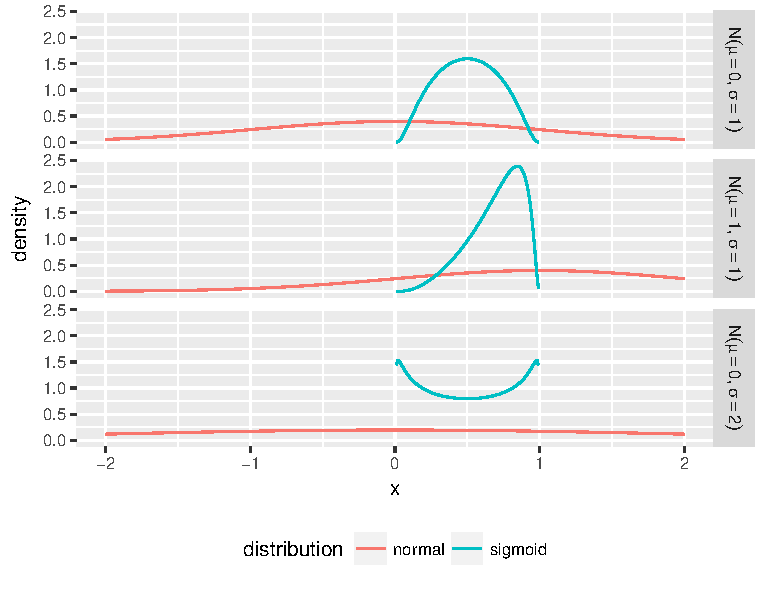
\includegraphics[scale=1]{theory/batch-norm-activation-distribution}
	\caption{Shows $X \sim \mathcal{N}(\mu, \sigma)$ and $\mathrm{sigmoid}(X)$ calculated using the \textit{change of variable theorem}.}
	\label{fig:convergence:batch-norm:activation-distribution}
\end{figure}

\subsubsection{A solution}
The \textit{internal covariate shift} issue can in practice be solved by using a small learning rate. However, this is not an optimal solution as it prolongs the optimization. Batch normalization is an alternative solution, that solves the issue by standardizing the input to the activation function. To truly standardize this input the covariance matrix, as well as its inverse square root, should be calculated. These calculations are very expensive, thus batch normalization makes a practical compromise by only standardizing using the variance.
\begin{equation}
\hat{z}_{h_\ell} = \frac{z_{h_\ell} - \mathbb{E}[z_{h_\ell}]}{\sqrt{\textsc{Var}[z_{h_\ell}] + \epsilon}}, a_{h_\ell} = \theta(\hat{z}_{h_\ell})
\end{equation}

The expectation ($\mathbb{E}[z_{h_\ell}]$) and variance ($\textsc{Var}[z_{h_\ell}]$) themselves are expensive to estimate over the entire dataset, thus it's only done over each mini-batch. This also makes it much more feasible to integrate the standardization into the backward pass. Note also that because the expectation is subtracted, the bias $b_{h_\ell}$ in $z_{h_\ell}$ has no effect and should thus be omitted:
\begin{equation}
z_{h_\ell} = \sum_{h_{\ell-1}}^{H_{\ell-1}} w_{h_{\ell-1}, h_\ell} a_{h_{\ell-1}} 
\end{equation}


Finally, to allow batch normalization to become the identity function, two more parameters ($\gamma, \beta$) are added to the optimization problem:
\begin{equation}
\hat{z}_{h_\ell} = \gamma_{h_\ell} \frac{z_{h_\ell} - \mathbb{E}[z_{h_\ell}]}{\sqrt{\textsc{Var}[z_{h_\ell}] + \epsilon}} + \beta_{h_\ell}, a_{h_\ell} = \theta(\hat{z}_{h_\ell})
\label{eq:theory:convergence:batch-norm}
\end{equation}

The backward pass for learning ($w, \gamma, \beta$) is rather complicated, but computationally completely feasible as long as the mini-batch size is small. See Appendix \ref{appendix:backward-pass:batch-norm} for the backward pass.

In the special case that $\theta(\cdot)$ is multiplicative linear with respect to a scalar (i.e. $\theta(\alpha \hat{z}_{h_\ell}) = \alpha \theta(\hat{z}_{h_\ell})$) and the following layer isn't sensitive to a multiplication factor, then $\gamma_{h_\ell}$ can be removed from the optimization. A common case is where $\theta(\cdot)$ is the ReLU function, in this case:
\begin{equation}
\begin{aligned}
\alpha_{h_\ell} = \mathrm{ReLU}(\hat{z}_{h_\ell}) &= \gamma_{h_\ell} \mathrm{ReLU}\left(\frac{z_{h_\ell} - \mathbb{E}[z_{h_\ell}]}{\sqrt{\textsc{Var}[z_{h_\ell}] + \epsilon}} +  \frac{1}{\gamma_{h_\ell}}\beta_{h_\ell}\right)\\
&= \gamma_{h_\ell} \mathrm{ReLU}\left(\frac{z_{h_\ell} - \mathbb{E}[z_{h_\ell}]}{\sqrt{\textsc{Var}[z_{h_\ell}] + \epsilon}} +  \tilde{\beta}_{h_\ell}\right)
\end{aligned}
\end{equation}

In the next layer $\alpha_{h_\ell}$ is then multiplied by some other weight that $\gamma_{h_\ell}$ can be merged into. This simplification can often be applied and can be quite valuable as it removed some computations and further simplifies the loss curvature.

\subsubsection{Inference}

With an established backward pass, the network can easily be trained. However, there is still an open question about how inference should be done.

The inference should be deterministic once training is done, thus the ideal solution would be to use the estimated expectation and variance from the entire training dataset in \eqref{eq:theory:convergence:batch-norm}. However, because this calculation can be rather expensive a more practical solution is to use a moving average. Let's denote $\sigma^2_{\mathcal{B}_i}$ and $\mu_{\mathcal{B}_i}$ as the variance and mean estimate after mini-batch $i$. Then in addition to the optimization of ($w, \gamma, \beta$), $\sigma^2_{\mathcal{B}_i}$ and $\mu_{\mathcal{B}_i}$ will also update during training.
\begin{equation}
\begin{aligned}
\sigma^2_{\mathcal{B}_i} &= \lambda \sigma^2_{\mathcal{B}_{i-1}} + (1 - \lambda) \textsc{Var}[z_{h_\ell}] \\
\mu_{\mathcal{B}_i} &= \lambda \mu_{\mathcal{B}_{i-1}} + (1 - \lambda) \mathbb{E}[z_{h_\ell}]
\end{aligned}
\end{equation}

At inference $\hat{z}_{h_\ell}$ are then calculated using $\sigma^2_{\mathcal{B}_i}$ and $\mu_{\mathcal{B}_i}$.

\begin{equation}
\hat{z}_{h_\ell} = \gamma_{h_\ell} \frac{z_{h_\ell} - \mu_{\mathcal{B}_i}}{\sqrt{\sigma^2_{\mathcal{B}_i} + \epsilon}} + \beta_{h_\ell}, a_{h_\ell} = \theta(\hat{z}_{h_\ell})
\end{equation}

\subsubsection{Weight sharing network}

Because it is the weight changes that causes an \textit{internal covariate shift}, the normalization should happen over all $z_{h_\ell}$ values that use these weights. Thus in RNN, the normalization should also be done over time, and in CNN the normalization should also happen over the ``image''. This works well for actual images, however in RNN and CNN that describes a causal relation, the mean and variance at any time step (e.g. $t=0$) will contain information from all time steps, which breaks the causality of the network. This issue in practice be solved by not normalizing over time, however, if the sequences aren't all of the same lengths then the mean and variance estimation for the last time step will be extremely poor.

\subsection{Layer Normalization}

Layer normalization attempts to solve the issues that exist when batch normalization is applied to causal weight sharing networks. It does this by not normalization over the batch, but normalizing over the $\{z_{h_\ell}\}_{h_\ell=1}^{H_\ell}$ vector. \cite{layer-normalization}

\begin{displayquote}
Notice that changes in the output of one layer will tend to cause highly correlated changes in the summed inputs to the next layer, especially with ReLU units whose outputs can change by a lot. This suggests the “covariate shift” problem can be reduced by fixing the mean and the variance of the summed inputs within each layer. \todo{understand this}
\end{displayquote}

Normalizing over the summed inputs $z_{h_\ell}$ results in the following forward pass:
\begin{equationbox}[H]
Activation:
\begin{equation*}
\begin{aligned}
z_{h_\ell} &= \sum_{h_{\ell-1}}^{H_{\ell-1}} w_{h_{\ell-1},h_\ell} a_{h_\ell-1} \\
\hat{z}_{h_\ell} &= \gamma_{h_\ell} \frac{z_{h_\ell} - \mu_{\ell}}{\sqrt{\sigma_{\ell}^2 + \epsilon}} + \beta_{h_\ell} \\
a_{h_\ell} &= \theta\left(z_{h_\ell}\right)
\end{aligned}
\end{equation*}
Statistics:
\begin{equation*}
\begin{aligned}
\mu_{\ell} &= \frac{1}{H_\ell} \sum_{h_\ell}^{H_\ell} z_{h_\ell} \\
\sigma_{\ell}^2 &= \frac{1}{H_\ell} \sum_{h_\ell}^{H_\ell} (z_{h_\ell} - \mu_{\ell})^2
\end{aligned}
\end{equation*}
\caption{Forward equations for Layer Normalization.}
\end{equationbox}

Note that the bias $b_{h_\ell}$ is excluded here for a different reason than what was the case in batch normalization. In batch normalization $b_{h_\ell}$ was a constant and is thus removed when the mean is subtracted. In layer normalization, the mean is over $h_\ell \in [1, H_\ell]$ and thus $b_{h_\ell}$ is no longer a constant. However the original reasoning for layer normalization ``output of one layer will tend to cause highly correlated changes in the summed inputs'' \cite{layer-normalization}, does not include $b_{h_\ell}$ in ``summed inputs'' and thus the normalization should only happen over $\sum_{h_{\ell-1}}^{H_{\ell-1}} w_{h_{\ell-1},h_\ell} a_{h_\ell-1}$. As such $\hat{z}_{h_\ell}$ actually becomes
\begin{equation*}
\hat{z}_{h_\ell} = \gamma_{h_\ell} \frac{z_{h_\ell} - \mu_{\ell}}{\sqrt{\sigma_{\ell}^2 + \epsilon}} + b_{h_\ell} + \beta_{h_\ell},
\end{equation*}
but $ b_{h_\ell}$ then becomes redundant because of $\beta_{h_\ell}$.

The backward pass for learning ($w, \gamma, \beta$) is like in batch normalization a bit complicated, see Appendix \ref{appendix:backward-pass:batch-norm} for the backward pass.

Similar to batch normalization the $\hat{z}_{h_\ell}$ calculation can be simplified if $\theta(\cdot)$ is multiplicative linear (i.e. $\theta(\alpha \hat{z}_{h_\ell}) = \alpha \theta(\hat{z}_{h_\ell})$) and $\gamma_{h_\ell}$ can be merged into a weight in the following layer.

\subsubsection{Properties}

Batch normalization and layer normalization have somewhat similar properties, as shown in Table \ref{table:convergence:layer-norm:properties}. \textit{Weight matrix re-centering invariance} is likely the most important property, as bad weight matrix initialization is often the cause of slow convergence. 

\begin{table}[H]
\centering
\begin{tabular}{r|p{2cm} p{2cm} p{2cm} p{2cm}}
	           & Weight matrix re-scaling & Weight matrix re-centering & Dataset re-scaling& Dataset re-centering \\ \hline
	Batch norm & Invariant & No & Invariant & Invariant \\
	Layer norm & Invariant & Invariant & Invariant & No \\
\end{tabular}
\caption{Invariance properties when using batch or layer normalization. Also, note that batch normalization is invariant to \textit{Weight vector re-scaling} and layer normalization is invariant to \textit{Single training case re-scaling} \cite{layer-normalization}.}
\label{table:convergence:layer-norm:properties}
\end{table}

Another difference between batch and layer normalization is that in layer normalization it is not necessary to maintain a moving average over $\mu$ and $\sigma^2$ for inference, as these are estimated per observation.

\subsubsection{Experimental Results}

In the original paper \cite{layer-normalization} they showed that layer normalization outperforms batch normalization in RNNs. batch normalization is however the preferred choice in CNN, though layer normalization still performs better than the non-normalized baseline. It is theoretically unclear why layer normalization performs poorly on CNNs, but a possible explanation is that there is an underlying assumption that the hidden units $a_{h_\ell}$ make similar contributions, in CNN the hidden units typically represents very different things (e.g. ear, mouth, hair) thus some will be very inactive while others will be very active.

\subsection{Residual Learning}

The most sophisticated neural networks are typically rather deep networks with many layers, thus it is easy to think that ``deeper is better''. However it turns that this is not necessarily true. First of all, there is a vanishing/exploding gradient problem, but recently with good normalization and weight initialization, this is becoming less significant. It turns out that adding layers to a networks that already works well can degrade performance. This is not just a matter of overfitting as also the training error degrades \cite{residual-learning}.

In theory, if there are too many layers the network should optimize such that some of the layers simply becomes the identity function. However, even modern day optimizers are not able to find such a solution. Residual learning solves this problem, by changing the network architecture such that the optimization problem is easier to solve. If the desired function is denoted $\mathcal{H}(\mathbf{x})$, residual learning solves the issue by changing optimization problem such it should find $\mathcal{F}(\mathbf{x}) \defeq \mathcal{H}(\mathbf{x}) - \mathbf{x}$ instead. This is done by transforming the layer to be $\mathcal{F}(\mathbf{x}) + \mathbf{x}$.

\begin{figure}[H]
    \centering
    \begin{subfigure}[b]{0.4\textwidth}
        \centering
        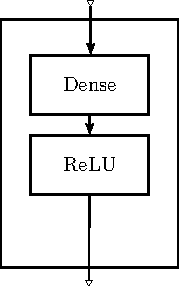
\includegraphics[scale=1]{theory/convergence-nonresidual-layer.pdf}
        \caption{Traditional Dense-ReLU layer}
    \end{subfigure}
    ~ %
    \begin{subfigure}[b]{0.4\textwidth}
        \centering
        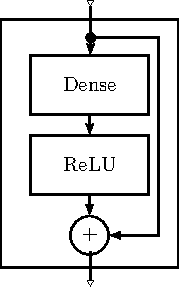
\includegraphics[scale=1]{theory/convergence-residual-layer.pdf}
        \caption{Residual Dense-ReLU layer}
    \end{subfigure}
    \caption{Comparison of traditional and residual Dense-ReLU layer}
\end{figure}

The idea is that getting $\mathcal{F}(\mathbf{x}) = 0$ is a lot easier to solve than $\mathcal{H}(\mathbf{x}) = \mathbf{x}$. For both the ReLU and sigmoid transformation, $\mathcal{F}(\mathbf{x}) = 0$ can be obtained by moving the weights to some extreme, while $\mathcal{H}(\mathbf{x}) = \mathbf{x}$ is drastically more difficult, particularly for the sigmoid case. If the layer really needs a non-trivial $\mathcal{H}(\mathbf{x})$ function, the optimizer simply needs to find $\mathcal{H}(\mathbf{x}) - \mathbf{x}$, which should not be that much more difficult.

A downside of using a residual layer is that the output dimension must match the dimension of $\mathbf{x}$. However there are workarounds, for example, one can add an extra dense layer to change the dimensionality of either the output dimension or $\mathbf{x}$.
\clearpage

\section{Sequential Networks}

Traditional Feed Forward Neural Networks are only capable of taking a fixed size vector as input and outputting a fixed sized vector. While it is theoretically possible to express a sentence in fixed sized vector by using a lot of zero padding, it is not very practical. A much better approach is to use sequential networks, these are able to take a variable length sequence of fixed sized vectors and outputting a sequence of fixed size vectors. There are different variations on this idea that utilizes different strategies of aligning the input sequence with the output sequence. The most general approach is called temporal classification \cite{alexgraves}, which allows any alignment between the input and target sequence. Temporal classification is necessary for language translation where the alignment often is unknown.

This class if problems are generally solved by creating a neural network that can fit the probability function $P(y_t | \{y_1, \dots, y_{t-1}\}, \{x_1, \dots x_{|S|}\})$, where $y_t\ \forall t \in [1, |T|]$ is the target sequence and $|T|$ is the length of the target sequence. Similarly $x_t\ \forall t \in [1, |S|]$ is the input (source) sequence of length $|S|$. The central idea is that the $P(y_t| \cdot)$ known the entire input sequence, but only the parts of the output sequence that came before $y_t$. This allows one to predict the entire sequence during inference, by iterating from $t = 1$ to $t = |T|$.

In training the loss is constructed by considering the joint probability over all time steps \cite{alexgraves}:
\begin{equation}
P(y_1, \dots, y_{|T|}) = \prod_{t=1}^{|T|} P(y_t | \{y_1, \dots, y_{t-1}\}, \{x_1, \dots, x_{|S|}\})
\end{equation}

This construction is computationally convenient as it allows one to use log-probabilities instead of probabilities:
\begin{equation}
\log(P(y_1, \dots, y_{|T|})) = \sum_{t=1}^{|T|} \log(P(y_t | \{y_1, \dots, y_{t-1}\}, \{x_1, \dots, x_{|S|}\}))
\end{equation}

The ByteNet model, which will be discusses later in section \ref{sec:theory:bytenet}, is able to fit the probability $P(y_t | \{y_1, \dots, y_{t-1}\}, \{x_1, \dots, x_{|S|}\})$. To understand the pros of ByteNet and how it differs from existing word-based neural translation models, a short introduction to two popular models, Sutskever 2014 \cite{sutskever-2014-nmt}, and Bahdanau 2015 \cite{bahdanau-2015-nmt} is given. Later in the ByteNet chapter the corns will be discussed.

\subsection{Sutskever Model}

\begin{equationbox}[H]
\begin{equation*}
\begin{aligned}
\text{encoding:} & \\
& \mathbf{h}_j = f(\mathbf{x}_j, \mathbf{h}_{j-1}) \quad \forall j \in [1, |S|] \\
\text{decoder:} & \\
&\mathbf{s}_i = \mathrm{g}(\mathbf{h}_{|S|}, \mathbf{s}_{i-1}) \\
&\mathbf{y}_i = \mathrm{softmax}(\mathbf{s}_i) \quad \forall i \in [1, |T|]
\end{aligned}
\end{equation*}
\caption{The Sutskever 2014 model \cite{sutskever-2014-nmt}.}
\end{equationbox}

The Sutskever 2014 model \cite{sutskever-2014-nmt} was one of the first neural machine translation models to shows state-of-the-art performance on the WMT 2014 dataset.

The general idea is to encode a sequences of words using a recurrent neural network, the last encoder state is then used to initialize the decoder. The decoder iterates using the previously predicted word. While this approach is mathematically elegant, encoding the source sentence ($S$) into a finite sized vector $h_{|S|}$ is in practice very difficult. The original implementation required a 8000 real valued dimensional vector for the sentence encoding. They also limited the source vocabulary to 16000 words and 8000 words for the target vocabulary.

Word-based neural machine translation models have shown to work well in practise, however they also have obvious limitations. Words not in the vocabulary can't be translated, a common issue is names which for character-based models are very easy to translate because they require no translation. The softmax of a large vocabulary is also expensive, in the original Sutskever implementation they used 4 GPUs for just the softmax and 4 more GPUs for the rest of the network. This again can be solved by using character-based models because the ``vocabulary'' is just the different letters, which there are a lot fewer off.

Using character instead of words in the Sutskever model may seam like a good idea at first, however the source and target sequences becomes much longer. Long sequences are difficult to encode and decode because the state is updated in each iteration, thus the state produced for the beginning of the sentence is easily forgotten. In theory LSTM units solves this vanishing-moment issue, but in practise it still exists. In particular Sutskever reversed the input sentence to get better performance, if there where no memory issues reversing the input sentence should have no effect.

\subsection{Bahdanau Attention Model}
\label{sec:theory:sequential:bahdanau}

\begin{equationbox}[H]
\begin{equation*}
\begin{aligned}
\text{encoding:} & \\
& \mathbf{h}_j = f(\mathbf{x}_j, \mathbf{h}_{j-1}) \quad \forall j \in [1, |S|] \\
\text{attention:} & \\
& e_{ij} = a(\mathbf{s}_{i-1}, \mathbf{h}_j) \\
& \bm{\alpha}_i = \mathrm{softmax}(\mathbf{e}_i) \\
& \mathbf{c}_i = {\textstyle \sum_{t=1}^T} \alpha_{it} \mathbf{h}_t \\
\text{decoder:} & \\
&\mathbf{s}_i = \mathrm{g}(\mathbf{c}_i, \mathbf{s}_{i-1}) \\
&\mathbf{y}_i = \mathrm{softmax}(\mathbf{s}_i) \quad \forall i \in [1, |T|]
\end{aligned}
\end{equation*}
\caption{The attention based Bahdanau 2015 model \cite{bahdanau-2015-nmt}.}
\end{equationbox}

Bahdanau et. al. solved this memory issue by letting the decoder look at selected parts of the encoding state sequence. It does this though what is called an attention mechanism. The attention $\bm{\alpha}_i$ is a weight vector, that is used in a weighted mean calculation over the encoded states $\mathbf{h}_t$. The weights a calculated using a sub-network that depends on the previous output state $\mathbf{s}_{i-1}$ and the encoding states. The weighted mean is then used to calculate the next output state $\mathbf{s}_{i}$.

The attention mechanism essentially recalculate a new encoding vector for each output state. This creates what called a resolution preserving encoding, that is an encoding which size depends on the source sequence, this is different from the Sutskever model that uses a fixed sized vector. The Bahdanau et. al model is words-based and achieved state-of-the-art like performance. On the surface there is nothing that prevents the Bahdanau et. al. model from being character-based, but by looking at the computational complexity it becomes clear that using characters is not a viable solution.

In each iteration on the output sequence, the attention model needs to calculate the weighted mean over the encoding sequence, this takes $\mathcal{O}(|S|)$ time. These calculations can not be reused in the next iteration because they also depends on the output state from the previous iteration $s_{i-1}$. The attention thus needs to be recalculated for each output state, resulting in a computational complexity of $\mathcal{O}(|S||T|)$.

Having this quadratic-like computational complexity $\mathcal{O}(|S||T|)$, means that using characters instead of words dramatically increases the running time.

\clearpage

\section{ByteNet}
\label{sec:theory:bytenet}

The ByteNet model is an alternative approach to neural machine translation, it specifically focuses on having linear computational complexity, having a resolution preserving encoding, and be a character-level translation model \cite{bytenet}. This is somewhat different from existing popular models such as the Sutskever 2014 model \cite{sutskever-2014-nmt} and the attention based Bahdanau 2015 model \cite{bahdanau-2015-nmt}.

Note that the model presented here is a simplified version of the original ByteNet model \cite{bytenet}. First, there are no bags of characters, only individual characters are used as the sentence representation. Secondly, the Sub-Batch normalization in the decoder is replaced by Layer Normalization, besides being a simpler solution than Sub-Batch Normalization this could also improve the model performance \cite{layer-normalization}.

\subsection{ByteNet Residual Block}

Before explaining the full ByteNet network, a central component of the ByteNet model called the \textit{ByteNet residual block} needs to be explained first. There are two variations of this an \textit{Encoder Residual Block}, and a \textit{Decoder Residual Block}. First the encoder version is explained and then some slight alterations of this will turn it into the decoder version. For a visual representation see Figure \ref{fig:bytenet:residual-block}.

\begin{figure}[h]
    \centering
    \begin{subfigure}[b]{0.45\textwidth}
        \centering
        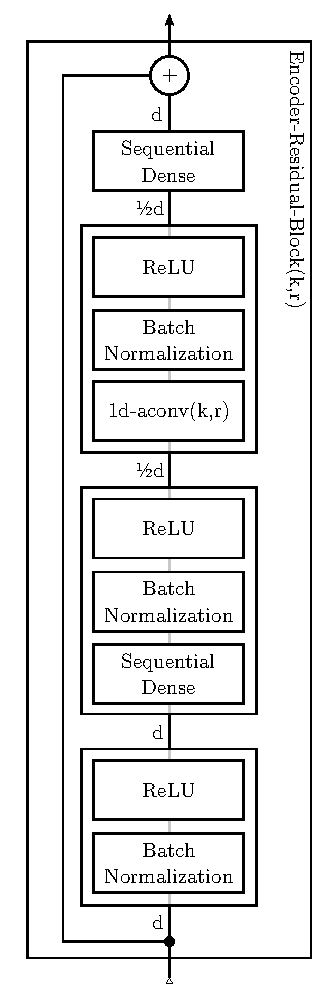
\includegraphics[scale=1]{theory/bytenet-residual-block.pdf}
        \caption{Residual Block used in encoder.}
    \end{subfigure}
    ~ %
    \begin{subfigure}[b]{0.45\textwidth}
        \centering
        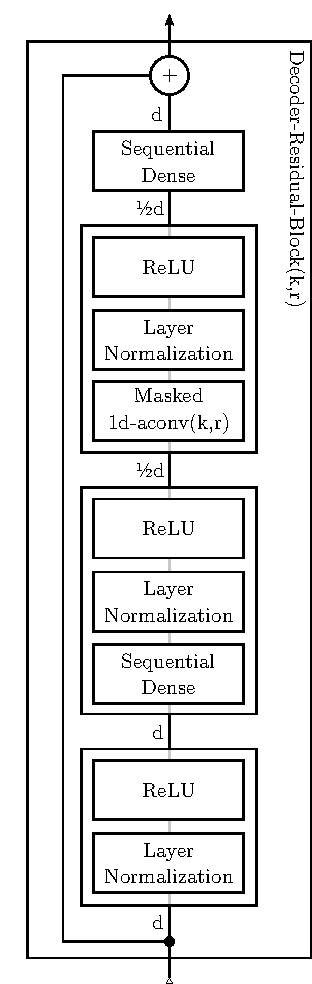
\includegraphics[scale=1]{theory/bytenet-residual-block-causal.pdf}
        \caption{Residual Block used in decoder.}
    \end{subfigure}
    \caption{The residual blocks used in the ByteNet model. The blocks are denoted by Encoder-Residual-Block$(k,r)$ and Decoder-Residual-Block$(k,r)$, where $k$ is the kernel width and $r$ is the dilation rate.}
    \label{fig:bytenet:residual-block}
\end{figure}

\subsubsection{Encoder Residual Block}

The \textit{ByteNet residual block} is at its core a dilated convolution, but adds upon this many of the ideas presented in section \ref{sec:convergence}. The entire block is a \textit{residual layer}, meaning that that the input is added to the final output of the transformation function $\mathcal{F}$. The transformation can be logically grouped into a set of sub-blocks, a normalization block, a dimensional reduction block, a dilated convolution block, and finally a dimensional restoration block.

The normalization block consists of Batch-Normalization and a ReLU activation. For this to make sense there must be some parameters before the activation such that the network can control the ReLU. This will either be an embedding lookup or another \textit{residual block}.

The dimensional reduction block reduces the dimensionality of the dataset from $d$ dimensions to $\frac{1}{2}d$ dimensions. This is done though the usual Dense Layer, Batch-Normalization, and ReLU activation block sequence. Note that the input is a sequence of vectors, a vector for each character, thus the dense matrix multiplication is performed on each vector in the sequence. This can also be described as a normal convolution with a kernel width of one.

\afterpage{\clearpage}

The dilated convolution block depends on two parameters (or 3 if dimension size $d$ is included), the kernel width $k$ and the dilation rate $r$. ByteNet specifies a specific structure for these parameters, but these choices only make sense from the full network perspective, thus they will be discussed later. Besides being a dilated convolution the sub-block is quite normal, as it also performs a batch-normalization and ReLU activation. The convolution also maintains the dimensionality, which at this point is $\frac{1}{2}d$.

For the \textit{residual layer} to make sense, the output dimension must be equal to the input dimension, thus the final sub-block is just a dense layer that transforms from $\frac{1}{2}d$ dimensions to $d$ dimensions. This sub-block does not contain either a Batch-Normalization, or a ReLU activation. Though these are implicitly performed if another \textit{residual block} follows.

\subsubsection{Decoder Residual Block}

The decoder is very similar to the encoder, the differences exist such that the decoder can't look into the future of the target sequence. If the decoder was allowed to look into the future it would be impossible to perform inference, when the target sequence is unknown. To prevent future inspection two changes are made‚ the dilated convolution is masked, and Batch-Normalization is replaced with Layer-Normalization.

Masking the convolution means that only the part of the convolution kernel that looks at the past is preserved. This is equivalent to fixing the right side (the future side) of the preserved kernel to zero.

\subsection{Hierarchical Dilated Convolution}
\label{sec:theory:bytenet:hierarchical-dilated-convolution}

Each \textit{ByteNet Residual Block} can conceptually be seen as just a modified dilated convolution. This conceptual model is useful for understanding the main trick that makes \textit{ByteNet} so powerful, \textit{Hierarchical Dilated Convolution}.

The idea behind \textit{Hierarchical Dilated Convolution} is that by exponentially increasing the dilation rate in stacked dilated convolution layers, the effective kernel width will exponentially increase for each layer, while the amount of weight in the kernel only increases linearly. The encoder part (bottom half) of figure \ref{fig:bytenet:simplified-hdc} helps to understand this idea in detail.

\begin{figure}[h]
    \centering
    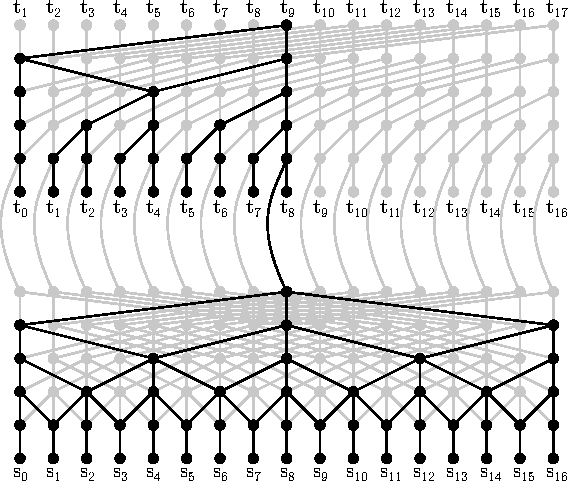
\includegraphics[scale=1]{theory/bytenet-hierarchical-dialted-convolution-enc-dec.pdf}
    \caption{A simplified version of the ByteNet model, showing the interaction between the decoder and encoder.}
    \label{fig:bytenet:simplified-hdc}
\end{figure}

Let the dilation rate for the encoding layers $\ell \in [1, L_{enc}]$ be denoted $r_\ell$, the exponential increasing dilation rate used in the ByteNet model is then $r_\ell = 2^{\ell - 1}$. The top layer $(L_{enc})$ will thus have a width of $(k-1) 2^{L_{enc} -1} + 1$. The effective total width is slightly larger because the layer below has a width of $(k-1) 2^{L_{enc} - 2} + 1$. This pattern continues down to the first layer, resulting in an effective total width of:
\begin{equation}
\sum_{\ell = 1}^{L_{enc}} (k - 1) 2^{\ell-1} + 1 = (k - 1) (2^{L_{enc}} - 1) + 1
\end{equation}
The kernel size is however $k \times d$ for all layers, thus the total amount of weights is:
\begin{equation}
\sum_{\ell = 1}^{L_{enc}} k d = L_{enc} k d
\end{equation}

In the original ByteNet model they use 4 dilated convolution layers, each with a kernel width of $5$, this results in an effective kernel width of 125 characters (actually it is 373 character wide because they repeat the pattern 3 times). Having a wide but computationally cheap kernel is extremely important for a character-based translation model such as ByteNet. In an attention-based translation model, such as the Bahdanau model \cite{bahdanau-nmt} the width is in theory arbitrarily wide (though in practice very wide attention mechanisms works poorly), however as discussed previously this approach causes a quadratic computational complexity (section \ref{sec:theory:sequential:bahdanau}). By \textit{hierarchical dilated convolution} ByteNet manages to keep the complexity linear, while still having a very wide kernel. In practice sentences have a limited length and thus a hierarchical dilated convolution approach can be comparable to an attention approach. In the WMT 2014 en-de dataset, the longest sentences are 400 characters wide (Figure \ref{fig:bytenet:wmt-deen-density}).

\begin{figure}[h]
    \centering
    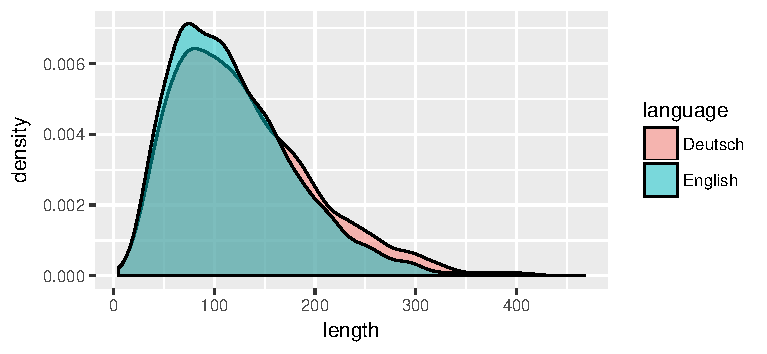
\includegraphics[scale=1]{theory/wmt-deen-density.pdf}
    \caption{Density estimate of the sentence length in the WMT 2014 en-de dataset.}
    \label{fig:bytenet:wmt-deen-density}
\end{figure}

\subsection{The Network}

The full \textit{ByteNet} model combines the \textit{Residual Blocks} with the \textit{Hierarchical Dilated Convolution} as discussed earlier. The \textit{Hierarchical Dilated Convolution} pattern is then repeated 3 times for both the encoder and decoder, as visualized in figure \ref{fig:bytenet:network}.

The input to the encoder is the source sequences mapped using an embedding matrix. The input to the decoder is the encoded sequence concatenated with the previous target prediction. This target prediction is then also mapped using a different embedding matrix. Note in particular that because the encoded vector is concatenated with the target sequence vector, the internal dimensionality of the decoder is twice that of the encoder. The decoded output is finally projected using a dense layer such the output has vocabulary sized dimensionality. After this, a softmax is used to transform the output into the probability domain.

An interesting effect of this network is that all layers are invariant to adding bias term. The encoder embedding and encoder layers are invariant because of Batch-Normalization. The decoder embedding and decoder layers are invariant because of Layer-Normalization. The final dense layer is invariant because of the following softmax.

\begin{figure}[H]
    \centering
    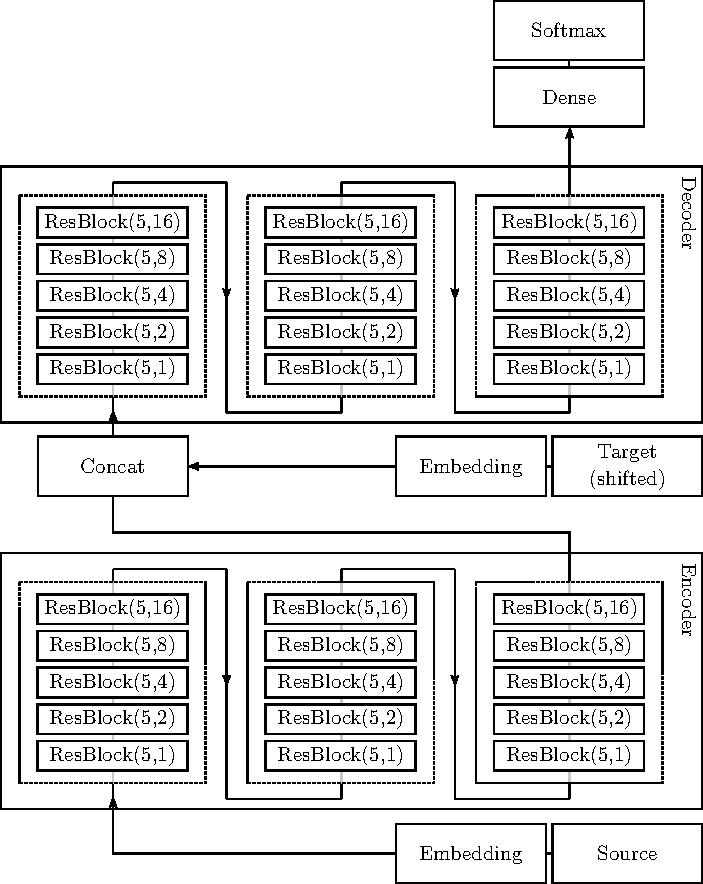
\includegraphics[scale=1]{theory/bytenet-network.pdf}
    \caption{The training network for the ByteNet Model, where the shifted target sequence is feed into the network. In the inference network, the shifted target sequence is replaced by the $\mathrm{argmax}(\cdot)$ of the softmax output. ResBlock$(k, r)$ in the encoder refers to the Encoder-Residual-Block$(k, r)$, in the decoder it refers to Decoder-Residual-Block$(k, r)$.}
    \label{fig:bytenet:network}
\end{figure}

\subsubsection{Training versus Inference}
The ByteNet model actually uses a different network for training than it does for inference. This is not strictly necessary, as one could use the same network for both training and interference like in an FFNN, however for sequential models the optimization can often converge faster if the target sequence is feed into the model.

Feeding the target sequence to the network is an optimization trick that may seem counter-intuitive at first. The idea is that because the prediction of the current character depends on the prediction of the previous characters ($\mathbf{y}_t = f(\mathbf{x}_{1:|S|}, \mathbf{y}_{1:t-1})$), then instead of letting the prediction cascade, which will also cause prediction errors to cascade, $\mathbf{y}_{1:t-1}$ is replaced with the known target sequence such that $\mathbf{y}_t = f(\mathbf{x}_{1:|S|}, \mathbf{t}_{1:t-1})$.

This trick also has the added benefit that training can be parallelized over target sentence and not just the observations and source sentence. 

\todo[inline]{There are some indications of this being suboptimal \url{https://arxiv.org/abs/1506.03099}}

\clearpage

\section{Semi-Supervised Learning for NMT}
\subsection{Semi-Supervised loss}
\subsection{Beam Search}
\clearpage